\section{Results} \label{sec:results}

\subsection{Micro Model}

Our micro model predicts that an increase in traffic flow at elevated traffic densities will be observed comparing human-driven traffic to half self-driven traffic and a further increase in traffic flow at elevated traffic densities will be observed as the saturation of self-driving cars in traffic increases to 90\%. These results can be seen in Figures \ref{fig:vel-plot} and \ref{fig:flow-plot}, which display the relationship between traffic density and traffic flux and traffic speed, respectively. 

\begin{figure}[h]
\centering
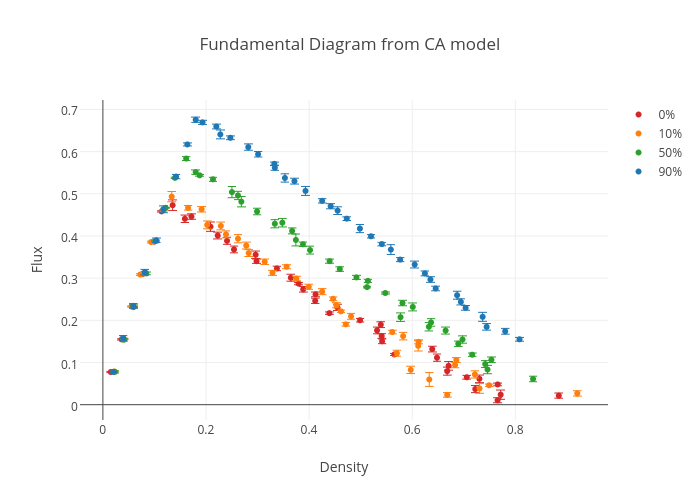
\includegraphics[width=0.6\textwidth]{img/flow-plot.png}\\
\caption{density and traffic flux data from our cellular automata model.}
\label{fig:flow-plot}
% \end{figure}

% \begin{figure}[h]
\centering
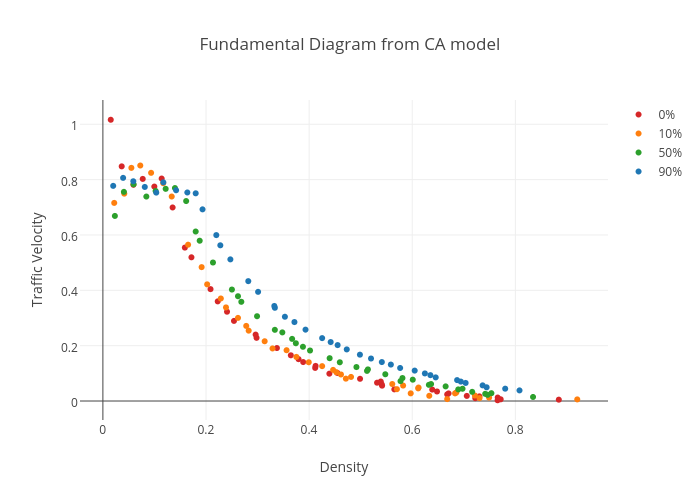
\includegraphics[width=0.6\textwidth]{img/velocity-plot.png}\\
\caption{density and velocity data from our cellular automata model.\\Each color represents different percentages of self-driven cars.}
\label{fig:vel-plot}
\end{figure}

Figure \ref{fig:flow-plot}, which visualizes the relationship between traffic flux and traffic density, reveals that an approximately 40\% increase in the maximal throughput of a road can can be realized through the widespread introduction of self-driving cars to the roadways. An approximately 20\% increase in maximal throughput of traffic can be realized through 50\% introduction of self-driving technology. Across different compositions of self-driving vehicles, flux is observed to be nearly identical up to $\rho_{crit}$ for human-driven traffic, approximately 34 cars per lane mile. Beyond that density, flux of traffic with self-driving cars begins to exceed the flux of human-driven traffic-- by a difference of constant magnitude for many density conditions. The magnitude of these difference greatly exceeds the variance that was observed in the data from stochastic simulation.

Figure \ref{fig:vel-plot} visualizes the relationship between traffic speed and density, for varying traffic compositions. Traffic speed is generally similar across the different traffic composition up to $\rho_{crit}$ for human-driven traffic. Beyond this point, the traffic speed of human-driven traffic begins to decline noticeably at greater density levels. The speed of mostly and partially self-driving traffic begins to decline at slightly greater densities but still is greater than that of human-driven traffic, with mostly self-driving traffic tending to move faster than partially self-driving traffic. The predicted traffic speeds become more similar across the spectrum of traffic composition, again, at high traffic density.

\subsection{Macro Model}

As mentioned in Section \ref{sec:macro_validation}, the macro level model of regional traffic patterns does not correspond well to observed peak volume traffic conditions in a quantitative sense. However, the model makes qualitative predictions that may be of interest to policy makers.

As would be expected, the model predicts that the introduction of self-driving cars do tend to ameliorate traffic jams. Our micro model does not predict a significant difference in traffic behavior between 0 and 10\% composition of self-driving cars in traffic. However, an effect on $\rho_{crit}$ was observed when the prevalence of self-driving cars grew to 50\% and, also, 90\%  (Section \ref{sec:macro_validation}). This difference in $\rho_{crit}$ predicted by the micro model was significant to observe reduction of traffic delays in the macro model. In all measured cases, the introduction of self-driving cars was observed to reduce or not affect travel times. 

However, widespread introduction of the self-driving car is no silver bullet. Under heavy traffic loads, trip times did indeed increase with 90\% self-driving traffic composition. For example, under average traffic conditions a trip down I-5 South is predicted to take 117 minutes. Under the maximum traffic load measured with no self-driving component of traffic, the duration of this trip increases to 169 minutes. However, at the maximum measured traffic load the trip is predicted to take only 145 minutes. Thus, the widespread introduction of self-driving cars has ameliorated -- but not eliminated -- traffic delays. Our model predicts that the introduction of self-driving cars has the potential to near completely eliminate -- at most -- minor traffic delays. Major traffic delays will likely not be completely eliminated by the introduction of self-driving cars, but -- even under the conservative assumptions of our models -- noticeably reduce traffic delays.

\noindent \begin{tabular}{
|p{3cm}||p{3cm}|p{3cm}|p{3cm}|p{3cm}|
}
 \hline
 \multicolumn{4}{|c|}{Predicted Effect of Percentage of Self-Driving Cars on Trip Times (Average Traffic)} \\
 \hline
Road & Trip Times for 0-10\% (min) & Trip Times for 50\%  (min) & Trip Times for 90\%  (min) \\
 \hline
 I-5 North    & 117.4 & 117.4 & 117.4 \\
 I-5 South    & 117.4 & 117.4 & 117.4 \\
 I-90 East    & 23.4 & 23.4 & 23.4    \\
 I-90 West    & 23.4 & 23.4 & 23.4    \\
 I-405 North  & 30.3 & 30.3 & 30.3    \\
 I-405 South  & 30.3  & 30.3 & 30.3    \\
 SR 520 East  & 12.8 & 12.8 & 12.8    \\
 SR 520 West  & 12.8 & 12.8 & 12.8    \\
 \hline
\end{tabular}

\bigskip

\noindent \begin{tabular}{
|p{3cm}||p{3cm}|p{3cm}|p{3cm}|
}
 \hline
 \multicolumn{4}{|c|}{Predicted Effect of Percentage of Self-Driving Cars on Trip Times (Peak Traffic)} \\
 \hline
 Road & Trip Times for 0-10\% (min) & Trip Times for 50\%  (min) & Trip Times for 90\% (min) \\
 \hline
 I-5 North    & 118.0 & 117.5 & 117.4  \\
 I-5 South    & 118.4  & 117.8 & 117.7  \\
 I-90 East    & 23.4 & 23.4  & 23.4   \\
 I-90 West    & 23.4 & 23.4 & 23.4   \\
 I-405 North  & 31.2  & 30.7 & 30.5  \\
 I-405 South  &  31.2 & 30.7 &  30.4 \\
 SR 520 East  & 12.9  & 12.8 & 12.8  \\
 SR 520 West  & 12.9  & 12.8 & 12.8  \\
 \hline
\end{tabular}

\bigskip

\noindent \begin{tabular}{
|p{3cm}||p{3cm}|p{3cm}|p{3cm}|
}
 \hline
 \multicolumn{4}{|c|}{Predicted Effect of Percentage of Self-Driving Cars on Trip Times (1.33$\times$ Peak Traffic)} \\
 \hline
 Road & Trip Times for 0-10\% (min) & Trip Times for 50\% (min) & Trip Times for 90\% (min) \\
 \hline
 I-5 North    & 121.4 & 119.0   & 118.1  \\
 I-5 South    & 123.6  & 120.3 & 119.2  \\
 I-90 East    & 23.7 & 23.5  &  23.4 \\
 I-90 West    & 23.7 & 23.5 & 23.4  \\
 I-405 North  & 33.6 & 32.2 & 31.7 \\
 I-405 South  & 33.5 & 32.2 & 31.7 \\
 SR 520 East  & 13.0  & 12.9 & 12.8  \\
 SR 520 West  & 13.0 & 12.9 & 12.8  \\
 \hline
\end{tabular}

\bigskip

\noindent \begin{tabular}{
|p{3cm}||p{3cm}|p{3cm}|p{3cm}|p{3cm}|p{3cm}|
}
 \hline
 \multicolumn{4}{|c|}{Predicted Effect of Percentage of Self-Driving Cars on Trip Times (1.5$\times$ Peak Traffic)} \\
 \hline
 Road & Trip Times for 0-10\% (min) & Trip Times for 50\% (min) & Trip Times for 90\% (min) \\
 \hline
 I-5 North    & 125.2  & 121.3  & 119.5 \\
 I-5 South    & 146.6  & 134.05   & 127.0  \\
 I-90 East    & 24.0 & 23.6 & 23.5  \\
 I-90 West    & 24.0  & 23.6 & 23.4   \\
 I-405 North  & 35.9 & 34.1 & 33.1   \\
 I-405 South  & 35.8  & 33.9 & 32.9   \\
 SR 520 East  & 13.2  & 13.0 & 12.9  \\
 SR 520 West  & 13.2  & 13.0 & 12.9  \\
 \hline
\end{tabular}

\bigskip

\noindent \begin{tabular}{
|p{3cm}||p{3cm}|p{3cm}|p{3cm}|p{3cm}|p{3cm}|
}
 \hline
 \multicolumn{4}{|c|}{Predicted Effect of Percentage of Self-Driving Cars on Trip Times (1.6$\times$ Peak Traffic)} \\
 \hline
 Road & Trip Times for 0-10\% (min) & Trip Times for 50\% (min) & Trip Times for 90\% (min) \\
 \hline
 I-5 North    & 127.7  & 123.1  & 120.8 \\
 I-5 South    & 169.0  & 154.4  & 145.0 \\
 I-90 East    & 24.2 & 23.7 & 23.6  \\
 I-90 West    & 24.2  & 23.8 & 23.5   \\
 I-405 North  & 41.5 & 36.0 & 34.5   \\
 I-405 South  & 40.7  & 35.8 & 34.2   \\
 SR 520 East  & 13.4  & 13.1 & 13.0  \\
 SR 520 West  & 13.3  & 13.0 & 13.0  \\
 \hline
\end{tabular}

\bigskip

\noindent \begin{tabular}{
|p{4cm}||p{3cm}|p{3cm}|p{3cm}|p{3cm}|p{3cm}|
}
 \hline
 \multicolumn{4}{|c|}{Predicted Effect of Percentage of Self-Driving Cars on Total Traffic Volume on Highways} \\
 \hline
  & 0-10\% Automated & 50\% Automated & 90\% Automated \\
 \hline
 Average Traffic  & 17657 & 17652 & 17652 \\
 Peak Traffic    & 34332  & 34062   & 33988 \\
 1.3$\times$ Peak Traffic  & 47741 & 46445  & 45922  \\
 1.5$\times$ Peak Traffic  & 57731  & 54784 & 53241 \\
 1.6$\times$ Peak Traffic  & 66119  & 61855 & 59754 \\
 \hline
\end{tabular}
